\chapter{本研究の目的}
\label{issue}

本研究ではソフトウェアの可読性を表すある1つの指標を対象とし、Swiftコンパイラにおいてその指標を改善することを目的とする。
本章では、ソフトウェアの可読性に影響を及ぼす要因を分類し、特に本研究で重要視する系統の要因を定量化することで、その指標の算出方法と正当性について述べる。


\section{ソースコード可読性中の改善すべき要因}
\label{issue:elements}

ソースコードの可読性に影響を与える要因には様々なものがあるが、本研究では可読性に関する過去の研究~\cite{elshoff}~\cite{banker-datar}~\cite{banker-davis}~\cite{tenny}~\cite{miara}に挙げられている要因を参考に、それらの要因を表~\ref{table:readability-elements}に上げる3つの系統へ分類する。

\begin{table}[!hbtp]
    \begin{center}
        \caption{ソースコード可読性に要因を与える要因の分類}
        \begin{listliketab}
        \begin{tabular}{|p{0.3\linewidth}|p{0.45\linewidth}|p{0.2\linewidth}|}
            \hline
            系統 & 分類される要因の例 & 可読性との関係 \\
            \hline
            \hline
            & \textbullet \ ソフトウェアに 使用されるデータ構造やアルゴリズムの複雑さ &\\
            ソフトウェアの処理の複雑性に関する要因 & \textbullet \ 制御構造などによるソフトウェアの実行パスの複雑さ & 複雑性が低いと可読性が上がる \\
            & \textbullet \ 使用されるプログラミング言語の表現力 &\\
            \hline
            & \textbullet \ コメントの充実度 &\\
            ソフトウェアの説明性に関する要因 & \textbullet \ 変数や関数、型などの名前の適切さ & 説明性が高いと可読性が上がる\\
            & \textbullet \ インデントの適切さ &\\
            \hline
            & \textbullet \ ソフトウェアが解決する問題の難易度 &\\
            ソフトウェアの読者に求められる知識量に関する要因 & \textbullet \ ソフトウェアが使用する手法の難易度 & 求められる知識量が少ないと可読性が上がる\\
            & \textbullet \ ソフトウェアに使用される手法の数 &\\
            \hline
        \end{tabular}
        \label{table:readability-elements}
        \end{listliketab}
    \end{center}
\end{table}

このように要因を分類することによって、~\ref{introduction:background}節で述べたSwiftコンパイラの可読性の低下がどのような要因によって起こりうるのかを考察できる。

まず、2つ目の説明性に関する要因については、コメントや識別子、インデントなどのプログラム中の明確に分離される部分が対象となっているため、既存のコードにそのスタイルを合わせたり、レビューで違いを指摘することが比較的容易である。
次に、3つ目の知識量に関する要因については、ソフトウェアの読者が誰であるかによって左右されるため、プロジェクトの発展に従って変化するようなものではない。
それらに対して、ソフトウェアの処理の複雑性は他の2つの側面と比較しても、特にレビューやコーディングスタイルへの追従によって保持することが難しく、今後Swiftコンパイラの可読性が低下する主要因となると考えられる。

そのため、本研究ではこれら3つの側面のうち特にソフトウェアの処理の複雑性を下げることによって得られる可読性の向上を重要視し、以降はそのための方法について論じる。


\section{ソフトウェアの処理の複雑性を定量化する手法}
\label{issue:method}

本研究が重要視するソフトウェアの処理の複雑性を定量化する手法は既存研究によって多く提案されている。

本節では、その中でも特によく取り上げられるLOC、FP、HCM、CCMという4種類の手法~\cite{yu}~\cite{symons}について整理する。
なお、これら4つの手法における値とソフトウェアの複雑性との関連性は全て、経験則的に示されているのみである。
そのため、実際に使用する際には単に値の大小を比べるだけでなく、その原因の救命までを含めた充分な考察を行うことが求められる。

\subsubsection{LOC (Line of Code)}

LOCではソフトウェアの実行可能なソースコードの行数を指標にソフトウェアの複雑性を算出する。
一般的に充分大きなソフトウェアでは行数の多いソフトウェアの方が複雑性が高くなるとされているが、小さなソフトウェアについては行数と複雑性の間の明確な相関は認められていないため、注意が必要である。

LOCは最も古典的でありながらもその扱いの容易さからよく用いられているが、特にプログラムの構造がその結果に一切反映されていない点については考慮する必要がある。

\subsubsection{FP (Function Point)}

FPは1979年にAllan J. Albrechtによって提案された。
ソフトウェアへ入出力されるデータとその入出力操作を列挙して重み付けを行い、その総和を指標にソフトウェアの複雑性を算出する。

FPは特に商用ソフトウェアの工数見積などの目的でよく使用されているが、対象とするソフトウェア内でのデータ処理による複雑性は経験的に決定される重み付け以外には一切反映されないため、データ処理中心のソフトウェアでは有意義な値にならない点に注意が必要である。

\subsubsection{HCM (Halstead Complexity Metrics)}

HCMは1977年にMaurice H. Halsteadによって提案された。
ソースコード中の演算子と被演算子の種類および数に基づく指標によってソフトウェアの複雑性を算出する。

HCMではデータフローに基づく複雑性を算出することができるとされているが、制御フローに基づく複雑性は一切勘案されていないため、分岐が1つもないプログラムと無限の分岐が存在するプログラムでも指標は同じ値となりうるなど注意が必要である。

\subsubsection{CCM (Cyclomatic Complexity Metric)}

CCMは1976年にThomas J. McCabeによって提案された。
ソースコード中の線形独立な経路の数を指標としてソフトウェアの複雑性を算出する。

CCMでは制御フローに基づく複雑性を算出することができるとされているが、データフローに基づく複雑性は一切勘案されないため、経路の数が同じであれば1文だけのプログラムと無限の文を持つプログラムでも指標は同じ値となりうるなど注意が必要である。

\vspace{2em}

このように、ソフトウェアの処理の複雑性を定量化する手法では各手法によって対象とすることのできるソフトウェアの種類が異なる。
そのため本研究においても、まずは各手法が本研究の対象とするSwiftコンパイラに対して有効であるかを検討する必要がある。


\section{本研究においてSwiftコンパイラの可読性を表す指標}
\label{issue:barometer}

本節では、~\ref{issue:method}節で述べた手法のうちどれをどのように使用することで本研究が対象とするSwiftコンパイラの複雑性を定量化できるかについて述べる。

Swiftコンパイラに各手法を適用する上で最も気をつけなければならないのは、Swiftコンパイラは様々な手法が用いられている大きなソフトウェアであるという点である。
どの手法であっても、コンパイラのように大きなソフトウェアの全体を対象として評価を行うと、部分部分では複雑性の高い箇所と低い箇所がそれぞれ存在しているにもかかわらず、それらが打ち消し合って平均的な結果のみしか算出できなくなってしまい、適切な考察に繋げられなくなってしまう。

また、コンパイラのソースコードの中にはコンパイラの基本的な機能を担う箇所と、特定の条件下のみで必要な機能を担う箇所が混在している。
本研究ではプロジェクトにおける拡張や修正の活発化に繋がるコンパイラの可読性を向上することが目的であるため、特によく読まれるであろう基本的な機能の複雑性から指標を算出するようにしたい。

これらの条件を満たすために、本研究ではSwiftコンパイラのソースコード中の基本的な一部の構文をコンパイルするために必要な箇所のみを対象に測定手法を用いることを考える。
しかし、例えばSwiftの基本的な構文を満たすいくつかのサブセットを定義し、その構文をコンパイルするために必要な箇所だけをソースコードから抜き出すようなことは到底簡単ではない。

そこで本研究においては、コンパイラ中の特定の構文を対象としている箇所を静的に決定するのではなく、その構文を実際にコンパイルした際に実行される箇所を動的に把握することで、特定の構文をコンパイルするために必要な箇所だけを対象とした複雑性の計測を行う。

表~\ref{table:evaluation-property}に、~\ref{issue:method}節の各手法について、Swiftコンパイラを対象とし(条件A)、さらにその中の特定の実行パスだけを抜き出したものを対象とする(条件B)という2つの条件下でも得られる値が充分に複雑性を表した指標となり得るかをまとめた。
LOCはその計測の容易さから部分的なプログラムでも正確に計測を行い、考察に繋げることができると考えられるが、他の手法はソフトウェア全体の複雑性を包括的に捉えることを目的としているため、本研究で用いるには適切とはいえない。

\begin{table}[!hbtp]
    \begin{center}
        \caption{各複雑性計測手法の本研究における条件との合致性}
        \begin{tabular}{|p{0.1\linewidth}|p{0.1\linewidth}|p{0.1\linewidth}|p{0.65\linewidth}|}
            \hline
            評価手法 & (条件A) & (条件B) & 理由\\
            \hline
            \hline
            LOC & ○ & ○ & 行数は対象に関わらず計測が可能である。\\
            \hline
            FP & × & × & コンパイラは入出力ではなく内部的な処理が中心となるため、FPの値はコンパイラの複雑性を充分表現できない。 \\
            \hline
            HCM & ○ & △ & プログラムの一部分だけを対象とした場合にHCMの値がどのような意味を示すかを慎重に考える必要がある。\\
            \hline
            CCM & ○ & × & プログラムの一部の実行パスだけを取り出すと、分岐の片方だけが実行されたプログラムでは分岐があるにも関わらず異なる実行パスが存在しないためにCCMに反映されず、CCMの値の意味が変化してしまう。\\
            \hline
        \end{tabular}
        \label{table:evaluation-property}
    \end{center}
\end{table}

そのため、本研究ではLOCに基づいて図~\ref{img:loc-measurement}のように特定のプログラムを実行した場合のコードだけを対象として計測を行い、それを本研究におけるSwiftコンパイラの可読性を表す指標として用いる。
この手順で計測された値は通常のLOCとは異なるため、これ以降区別するために実行部分LOCと呼ぶ。

\begin{figure}
    \begin{center}
        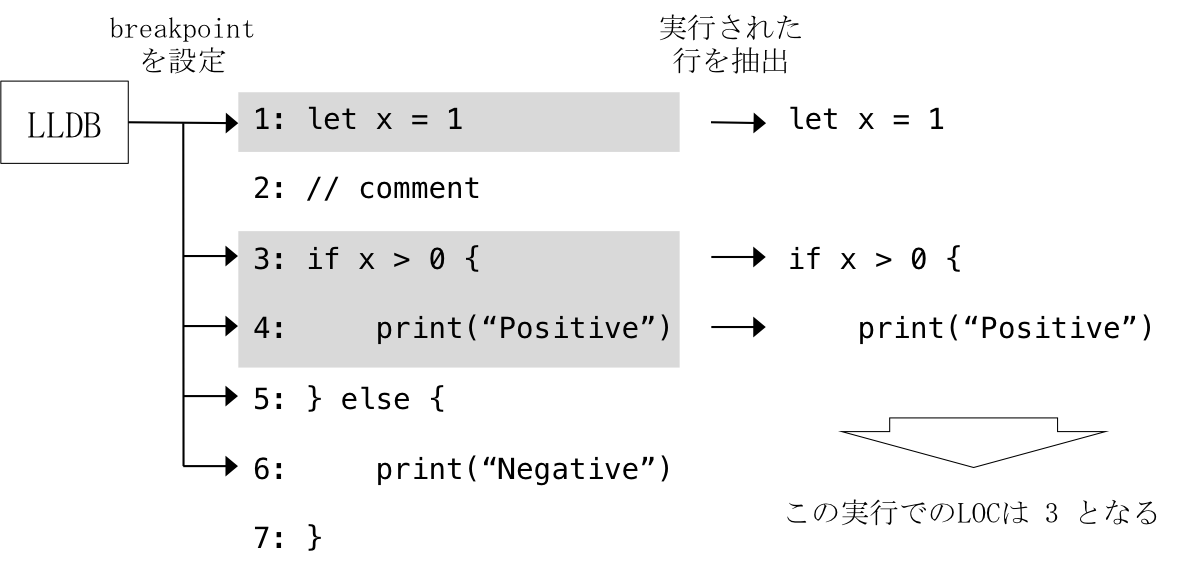
\includegraphics[scale=0.8]{./img/loc_measurement.png}
        \caption{実行部分LOCの計測手順}
        \label{img:loc-measurement}
    \end{center}
\end{figure}

つまり、本研究の目的はSwiftの基本的なプログラムを対象とした際のSwiftコンパイラの実行部分LOCを下げることであり、それが可読性の向上ひいてはプロジェクトの活性化に繋がるものであると考える。
